\chapter{Threat model}
\label{model}
In this chapter, we deepen several privacy weaknesses that affect the current version of the LoRaWAN protocol. First, we introduce the security policies adopted in designing LPWAN technologies. Next, we explain the security mechanisms of LoRaWAN and their flaws. Finally, analyzing the privacy-related problems of this protocol, we identify the object of study of this thesis, a threat associated with the analysis of two identifiers used in LoRaWAN devices.

\section{Security requirements}
Like other IoT technologies, the nature of the information produced, processed, transmitted in LPWANs has significant implications on network security. Confidentiality, Integrity, and Availability, otherwise known as the \textit{CIA} triad, are the three main security principles followed in developing the security of the LPWAN technologies \cite{AdefemiAlimi2020}: 
\begin{figure}[ht]
    \centering
    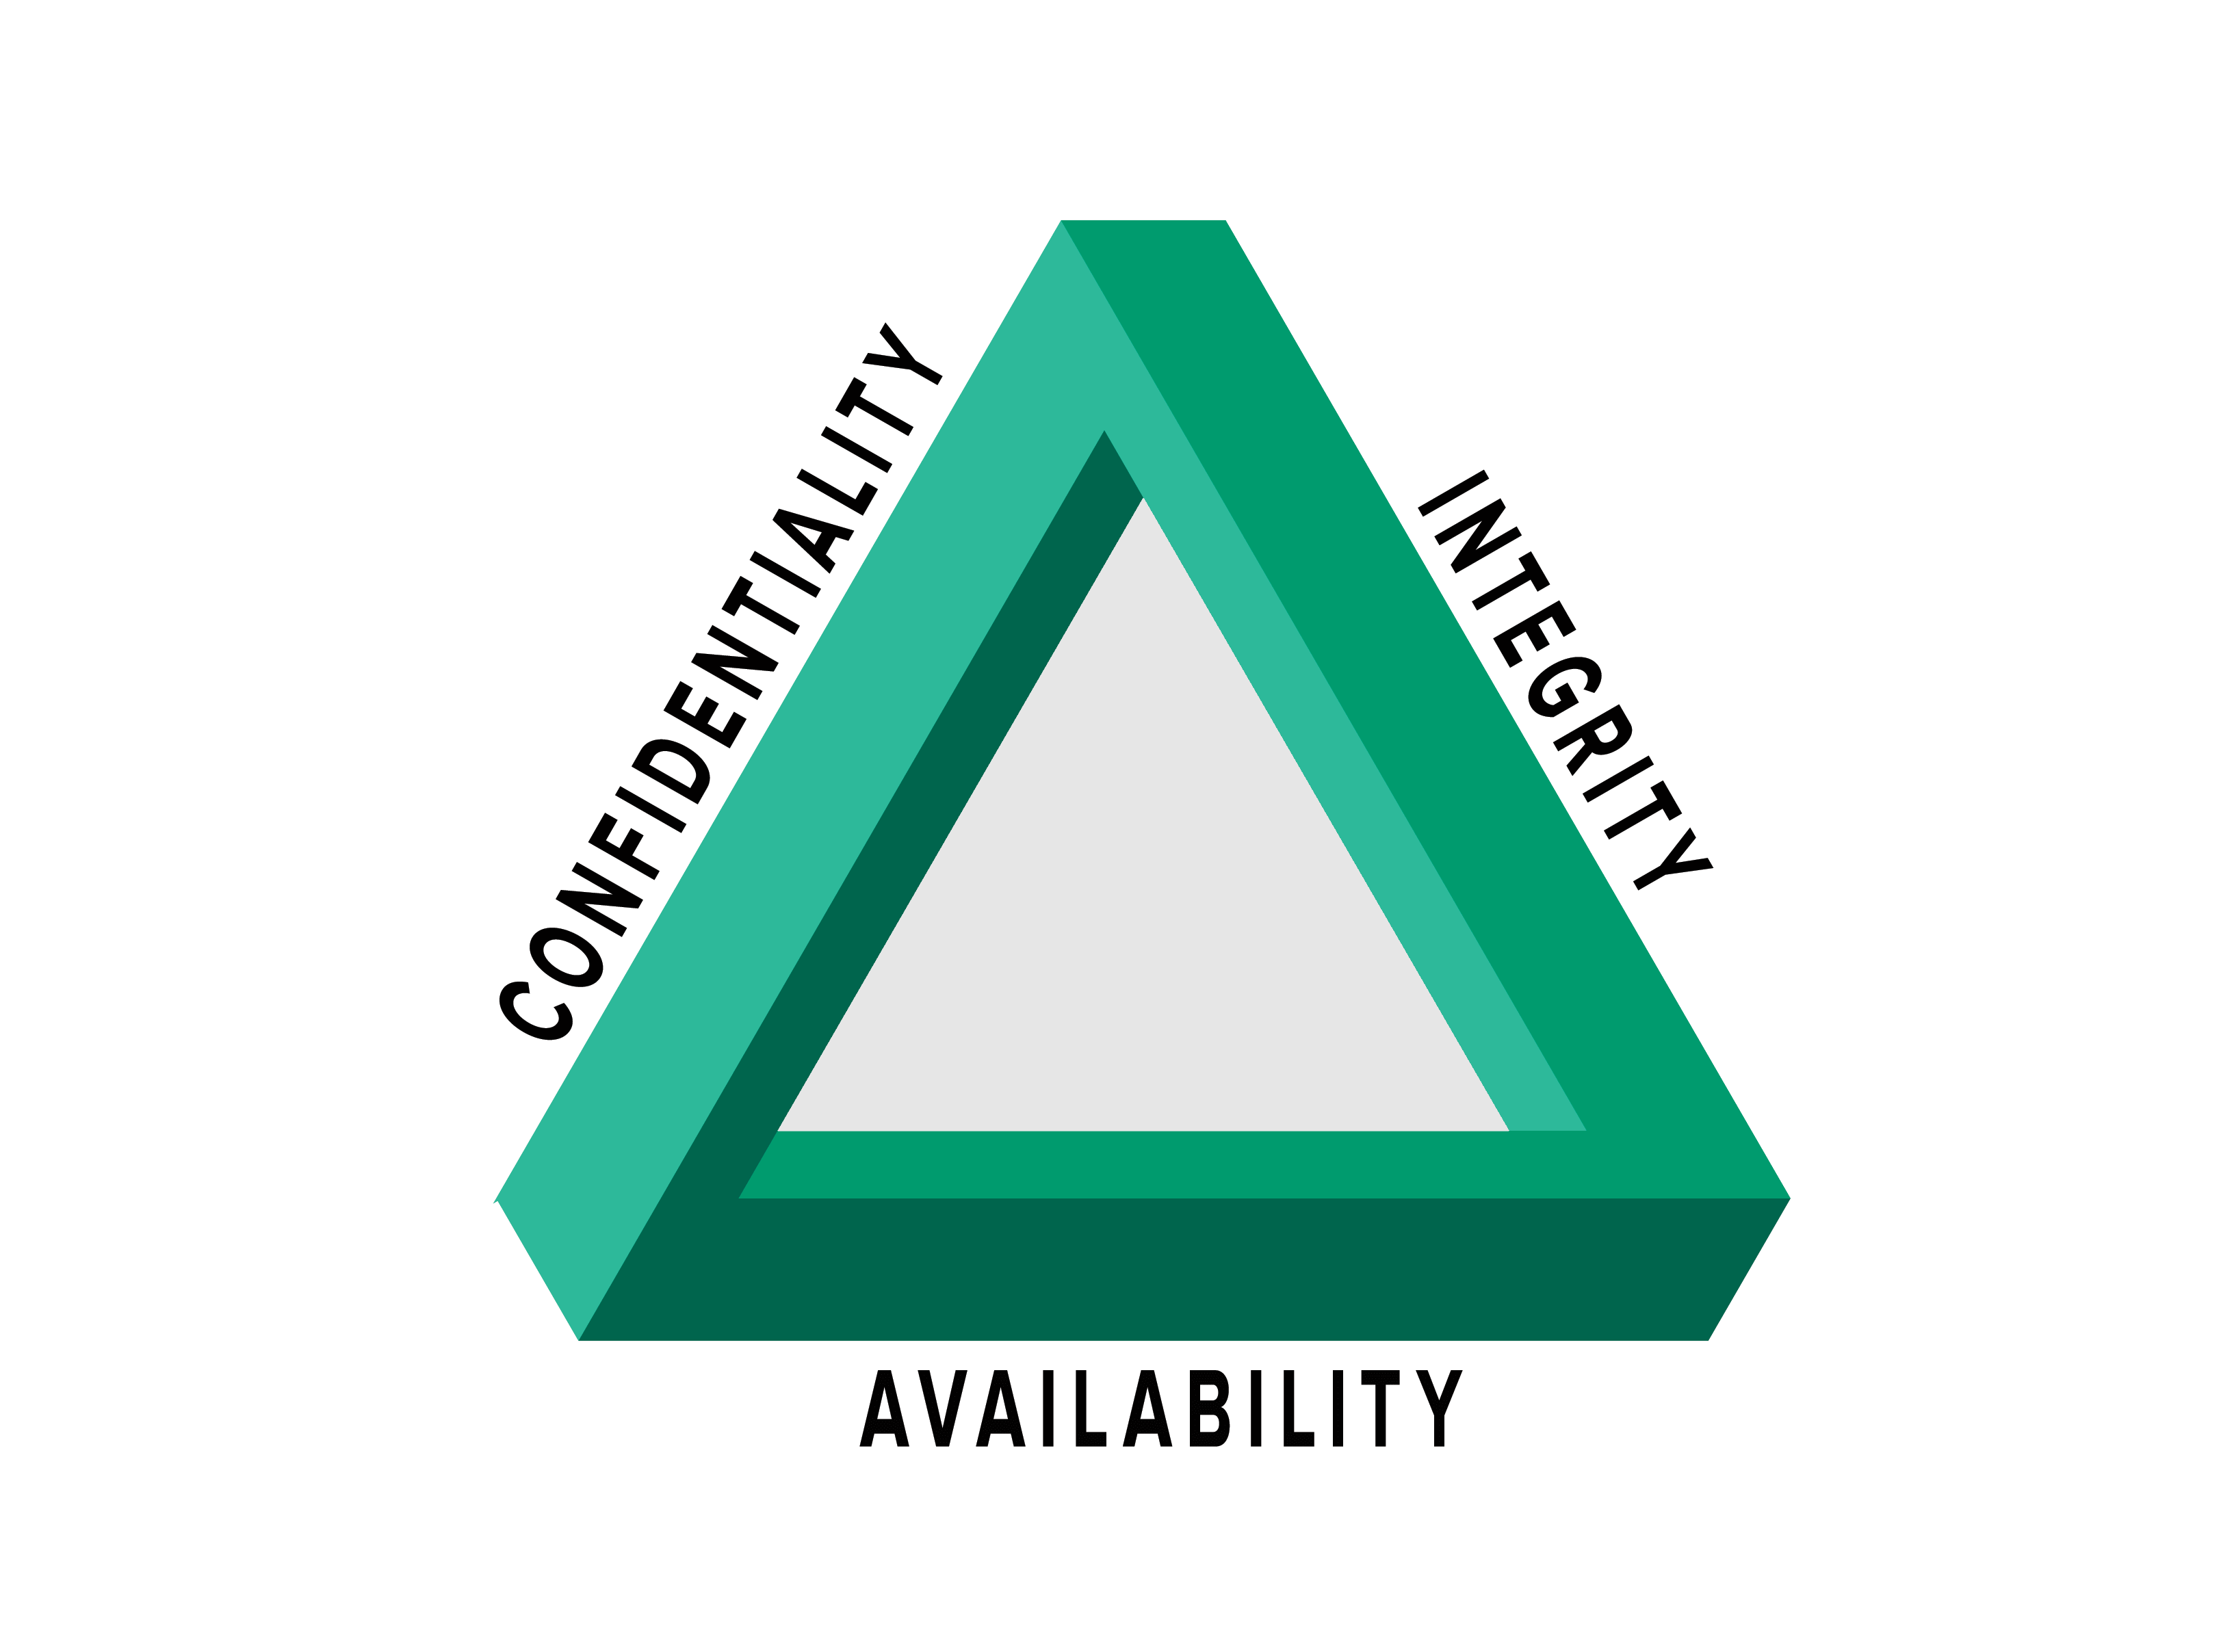
\includegraphics[width=0.5\linewidth]{images/threat/cia_triad.png}
    \caption{The CIA triad}
    \label{fig:triad}
\end{figure}

\begin{enumerate}
	\item \textit{Confidentiality}. It refers to a situation whereby the transmitted data are accessible only to the sender and the recipient. There are several ways to compromise the confidentiality, such as the well-known Man-In-The-Middle (MITM) technique, where the attacker furtively alters the communications between two nodes.
	\item \textit{Integrity}. Data integrity is what the \textit{I} in CIA Triad stands for. It refers to the protection of network data, preventing unintentional or intentional alteration of the information by unauthorized intruders. Typical integrity attacks performed on LPWANs are the replay attack and the wormhole attack \cite{Chacko_2018}. The replay attack happens when a valid packet transmission is maliciously manipulated. The wormhole attack consists of a situation whereby an intruder receives network packets at one location, forwards them to another node, and continues to replay the packets within the entire network. Often the wormhole attack is be performed using two devices, the sniffer and the jammer. While the sniffers capture the network packets, the jammer blocks or interference with the communications.
	\item \textit{Availability}. This is the final component of the CIA Triad and refers to the actual availability of data. Network resources should be always obtainable for the authorized user when required. This requirement prevents bottleneck situations that hinder information flow. The most famous availability threat is Denial of Service (DoS) attacks, the attempt to consume network resources or bandwidth \cite{Al-Hadhrami2021}. Common DoS-related attacks include DNS flood, Internet Control Message Protocol (ICMP) broadcast, and SYN flood.
\end{enumerate}

\begin{table}
    \centering
    \label{tab:common_attacks}
    \caption{Common attack types in the CIA triad and their implications}
    \begin{adjustbox}{max width=1\textwidth,center}
        \begin{tabular}{|c|l|l|}
        \hline
        \textbf{Attack type}       & \textbf{Attack features}                                                                                                   & \textbf{Implications}                                                                                  \\ \hline
        \textit{Eavesdropping}     & Overhear and intercept data                                                                                                & Gain access to sensitive/private information                                                           \\ \hline
        \textit{Jamming}           & \begin{tabular}[c]{@{}l@{}}Intentional transmission to disrupt\\ communication\end{tabular}                                & \begin{tabular}[c]{@{}l@{}}Cut-off communication, causing\\ congestion, exhausting energy\end{tabular} \\ \hline
        \textit{Replay attack}     & Repeat a valid data transmission                                                                                           & Generate false messages, increase congestion                                                           \\ \hline
        \textit{Wormhole}          & \begin{tabular}[c]{@{}l@{}}Create low latency tunnel between two\\ malicious nodes\end{tabular}                            & Sending false or out-dated data                                                                        \\ \hline
        \textit{Man-in-the-middle} & \begin{tabular}[c]{@{}l@{}}Sniff network to intercept communication\\ between nodes\end{tabular}                           & Gain access to sensitive or private information                                                        \\ \hline
        \textit{Denial of service} & \begin{tabular}[c]{@{}l@{}}A general attack type that can include\\ multiple attacks happening simultaneously\end{tabular} & Disrupt normal operation of the network                                                                \\ \hline
        \end{tabular}
    \end{adjustbox}
\end{table} 

\subsection{Security in LoRaWAN}
Since devices are designed to last for many years, security plays a key role in the LoRaWAN protocol. The security design criteria follow the CIA triad and adopt the main LoRaWAN principles: low power consumption, low implementation complexity, and low-cost \cite{lorawan_security}. The fundamental properties are:
\begin{enumerate}
	\item Mutual authentication.
	\item Integrity protection. 
	\item Confidentiality.
\end{enumerate}
Mutual authentication, established between an ED and the network, ensures that only authorized devices can join authentic networks while MAC and application messaging are integrity-protected with two session keys, AppSKey and NwkSKey. As shown in Figure \ref{fig:encryption}, each payload, encrypted by AES-CTR, carries a frame counter to avoid packet replay and Message Integrity Code (MIC) to avoid packet tampering. This protection, combined with mutual authentication, ensures that network traffic is not altered, comes from a legitimate device, and is not comprehensible to eavesdroppers. 
\begin{figure}[H]
    \centering
    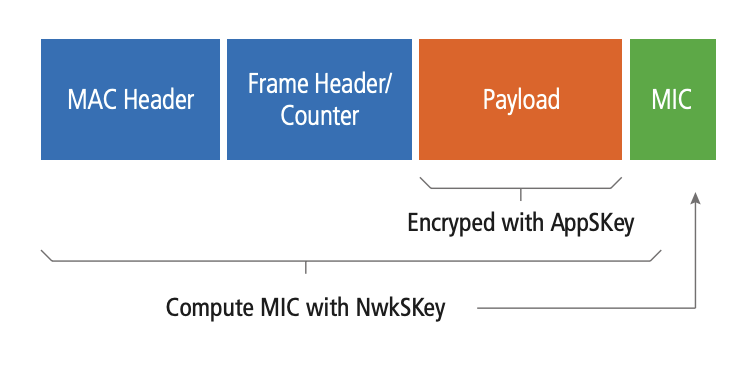
\includegraphics[width=0.7\linewidth]{images/threat/encryption.png}
    \caption{The encryption in LoRaWAN}
    \label{fig:encryption}
\end{figure}
Despite LoRaWAN being designed to be very secure with authentication and encryption mandatory, the 1.0 specification suffers from several security vulnerabilities, partially solved in the LoRaWAN 1.1. \cite{8117042}. The newest version of the protocol mainly combat confidentiality issues by making specification changes to the MAC layer but needs to be made to resolve integrity, availability, and authentication vulnerabilities. For example, LoRaWAN lacks in creating a secure channel between the Node Server and the Join Server. In addition, the PHY layer is prone to Denial-of-service attacks due to impersonation and jamming attacks \cite{9356425}. 


\section{Privacy threats}
As opposed to security, privacy aspects in LPWANs have received little attention. As shown in \ref{fig:passive}, since the long communication range of LPWAN technologies allows messages to be received several kilometers away, an eavesdropper can easily record sensitive information, even if located many hundred meters from endpoints.
\begin{figure}[ht]
    \centering
    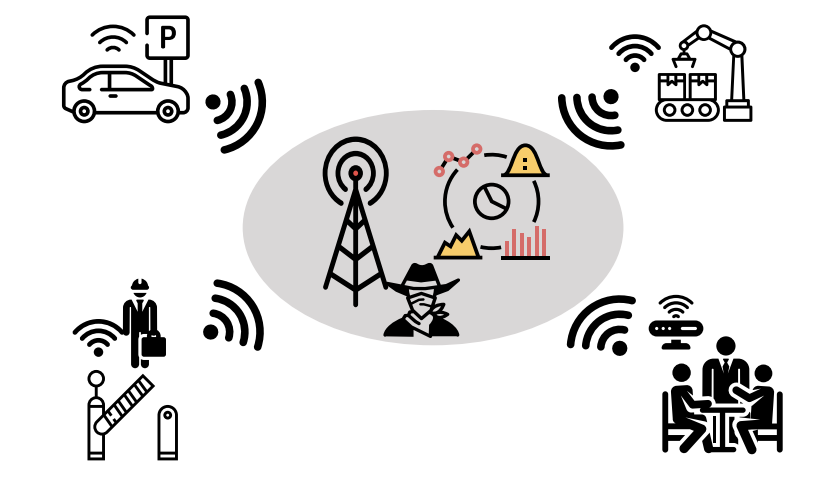
\includegraphics[width=0.7\linewidth]{images/threat/passive_adversary.png}
    \caption{When end devices transmit messages to the server, the passive adversary can easily collect sensitive information.}
    \label{fig:passive}
\end{figure}
By leveraging features of the raw wireless signal, attackers can interfere with the activities of devices operating in the network. In detail, we assume that the passive adversary, equipped with one or more receivers collecting end device transmissions, is within the communication range of at least one gateway and that it has a \textit{priori} knowledge about the application associated with an ED.  
\\
With these assumptions, the intruder can perform two relevant privacy-
related threats.

\begin{enumerate}
	\item\textbf{Fingerprinting}. Device Fingerprinting (DFP) denotes the set of techniques used to identify a device using the information extrapolated from the packets it uses to communicate over the network \cite{Gu2018}. DFP is commonly used in general-purpose devices to track user behavior and application usage. Interesting implementations include browser fingerprinting for web analytics, fraud detection, and accountability \cite{28180002818032}. Despite the benefits for the user experience, DFP poses also security and privacy risks. For example, LoRa devices can be uniquely recognized using physical (PHY) layer fingerprinting \cite{inproceedings}. It leverages on differences in the analog RF signals sent by wireless devices, caused by imperfections introduced in the analog hardware components during the manufacturing process \cite{10.1145/1409944.1409959}, demonstrating that an adversary can identify a transmitter independently of the modulation scheme or cryptographic mechanisms used.

	\item \textbf{Information leakages}. Since LPWAN is technology-constrained, attackers can easily reconstruct a view of the network they monitor. While other wireless devices transmit messages not necessarily related to real situations, LPWAN sensors are simpler and often dedicated to no more than one function, such as transmitting data when a given event occurs \cite{information_leakage}. Moreover, the LPWAN event space is small and binary, making the purpose of the individual sensors even clearer. Just consider the case of a parking system application that notifies clients if a given parking lot is occupied or not \cite{app10134674}. Endpoints send only two binary messages, the lot is empty or the lot is not empty, and only when there is a change of state (a vehicle left the lot). In absence of obfuscation techniques, a potential attacker recognizes the presence of real messages by simply eavesdropping on the LPWAN channel.
\\
In other scenarios, a deviation from standard transmission behavior presupposes the occurrence of an event. For example, in the case of an application that monitors the availability of a meeting room, the LoRa sensor transmits less when there is a series of long meetings that keep the room busy. The eavesdropper, collecting the messages in a given time frame, can use \textit{traffic analysis} techniques to extrapolate the transmission behavior and gain information about given circumstances.
\end{enumerate}

\subsection{Open issues}
\label{address_identification}
Even if the privacy aspects in LoRaWAN are not a new research topic, there are still open and unexplored problems in this context. As we have seen, LoRaWAN sensors are configured to have a very minimal behavior, causing common vulnerabilities, such as fingerprinting and information leakages. Despite the various countermeasures proposed and applied, there are still open issues that cause privacy-related matters. In this work, we focus on a threat correlated to two LoRaWAN identifiers, the \textit{DevAddr} and the \textit{DevEUI}. 

\subsubsection{Re-identififying addresses}
To avoid malicious fingerprinting, LoRaWAN doesn't expose to eavesdroppers sensitive information concerning devices and the network to which they are associated. For a given endpoint, only the application and the network knew the association between the current DevAddress and the DevEUI. Since DevEUI is revealed only during the OTAA procedure and the DevAddress is sent only in uplink messages, an ED can't send a packet with both identifiers exposed. 
\\
The decoupling of the DevEUI from the DevAddress guarantees devices' anonymity. Indeed, the NwkID field contained in the DevAddress reveals information about the network, and the OUI field of DevEUI contains information about the constructor of the device. By combining these two elements, the attacker increases its knowledge about the targeted LoRaWAN network. For example, it can determine which devices from a given operator (OUI) are around an assigned gateway (NwkID) or if the network belongs to private or experimental projects. Several studies demonstrate that the current LoRaWAN specification is not strong enough to assure that the association of these addresses remains unknown to unauthorized parts. For example, a technique proposed in \cite{tech2020} recognizes the DevAddress-DevEUI association relying on the timing between a Join-Request and the immediately following uplink message. The reidentification of these identifiers allows the discovery of peculiar activities in the network. By analyzing the traffic flow of Bouygues Telecom, this research demonstrates that during a peak in device activations, the newly joined devices are used only for test purposes.
\\
On the opposite, a second research \cite{devil} goes further: it underlines that this temporal linking is not always constant and proposes a pattern-based approach, named DEVIL, which, tested on a real dataset provided by an Italian operator, declares more accurate results. DEVIL is a batch-type algorithm: it processes all the data a posteriori, collecting uplink and join request messages in a given time window and elaborating them later.

\vspace{5mm}

As we have seen, pattern matching proves to be an effective strategy in detecting those devices whose pair \textit{DevAddr} - \textit{DevEUI} of identifiers can be easily recognized. In this thesis, we propose a defensive strategy that, exploiting the advantages of pattern matching, can prevent the re-identification attacks mentioned above.